\chapter{Introduction} \label{chap:intro}

The advent of blockchain technology has paved the way for decentralized finance (DeFi), offering a trustless and transparent financial ecosystem. Dharma Network emerges as a revolutionary decentralized application (DApp) built on the \textit{Algorand blockchain}\footnote{\href{https://developer.algorand.org}{Algorand blockchain} is a proof of stake layer 1 that is known to solve the "blockchain trilemma": decentralization, security and scalability}. \newline
It aims to work as a reward token inside distributed organizations incentivizing productivity and feedback, through blockchain and decentralized finance, creating a reward system based in a token that benefits all participants.\newline
At a first release, the application will connect to the GitHub API, extract the users' data and, upon the evaluation of such, the employee will be rewarded. 

\section{Contextualization} \label{sec:context}


This project was developed as part of the curricular internship between Yarilabs and the bachelor on Computer Systems Engineering, at IPCA.\newline

\href{https://www.yarilabs.com}{Yarilabs}\footnote{For further research on Yarilabs, go to: https://www.yarilabs.com} is known for its expertise in areas such as web and mobile application development, cloud computing and blockchain. By staying abreast of the latest industry trends and leveraging emerging technologies, Yarilabs is able to create tailored solutions that address the unique needs of each client.\newline

One of the key strengths of Yarilabs is their focus on collaboration and communication. They work closely with their clients throughout the development process, ensuring that the final product aligns with their vision and requirements. By fostering a collaborative environment, Yarilabs can effectively translate ideas into tangible solutions that drive business growth.\newline

In addition to their development services, Yarilabs also offers consulting and technical advisory services. Their team of experts can provide guidance on technology strategy, system architecture, and optimization, helping businesses make informed decisions that enhance their operations and competitive advantage.\newline

Yarilabs is the proud creator of \href{https://www.mydharma.network}{Dharma Network}\footnote{For further research on Dharma Network, go to: https://www.mydharma.network}, the project that will be exploited on this report.

\section{Purpose} \label{sec:purpose}

The purpose of Dharma Network is to create a trustable and fair ecosystem where users, developers and non-developers can mine DHARM, a utility token, through Proof-of-Real-Work (PoRW). By incentivizing users to engage in specific projects, Dharma Network aims to promote a decentralized system of wealth distribution and foster community participation.\newline

At the core of Dharma Network is the idea of creating a circular economy within a community, where rewards are distributed based on individual contributions and the evaluation of one's team. By implementing a transparent evaluation system, each team member's work is carefully assessed and a reward is calculated and distributed accordingly. This approach encourages collaboration and ensures that everyone's efforts are recognized and valued. \newline
Companies can use DHARM as a way to incentivize their users or employees, offering them rewards in the form of DHARM tokens. This can help to increase user engagement and loyalty, while also providing users with a tangible reward for their efforts.\newline

\section{Motivation} \label{sec:motivation}

Teams are key components of any project and organization, which is why it's an important factor to keep them safe, healthy and motivated. 
One of the easiest ways to keep them motivated is through rewards, and that's where Dharma Network gets in. It's a fun and modern token that motivates people and boosts their performances.\newline

In addition to its use as a reward, DHARM can also be used for governance purposes. Token holders have the ability to propose and vote on changes to the protocol, allowing for a more decentralized and democratic decision-making process.\newline

Dharma Network is driven by the vision of democratizing access to financial services and eliminating the need for intermediaries. By leveraging blockchain technology and decentralized applications, Dharma Network empowers individuals to participate in mining, govern the network and influence decision-making processes.

\subsection{Why should decentralized finance services be adopted?}

In recent years, decentralized finance (or DeFi) has emerged as a disruptive force in the financial industry. Built on blockchain technology (see section \ref{blockchain}), DeFi aims to provide an open, permissionless and inclusive financial system that operates without intermediaries. It encompasses a wide range of financial applications and services, such as lending, borrowing, decentralized exchanges, stablecoins and more. With its potential to revolutionize traditional financial systems, DeFi has garnered significant attention.

The adoption of decentralized finance services brings numerous benefits. Firstly, it enables greater financial inclusivity by removing barriers such as geographical limitations and minimum investment requirements. Secondly, decentralized finance provides increased transparency and immutability, reducing the risk of fraud and manipulation. Lastly, it allows users to retain control over their funds and eliminates the need for intermediaries, leading to reduced fees and enhanced financial sovereignty \cite{twp, cwi, coint}.

\subsubsection{Decentralized finance: a solution for global income inequality?}

\begin{enumerate}
    \item \textbf{The Challenge of Global Income Inequality}

Global income inequality is a pressing issue that affects billions of people worldwide. The wealth gap between the rich and the poor has continued to widen, exacerbating social and economic disparities. Traditional financial systems, characterized by centralized control and exclusionary practices, have played a role in perpetuating this inequality. Lack of access to banking services, high transaction fees and limited financial opportunities have hindered the economic progress of marginalized communities.

\begin{flushright}
   \textsl{''(...) As of 2022, the top 10\% of Americans hold nearly 70\% of the wealth in the United States. This means that 90\% of the country only takes home 30\% of the wealth. South Africa is another example, with the top 10\% taking home 65\% of the wealth.'' \cite{coint}} \\
\end{flushright}

\begin{comment}
    \vspace*{1cm}
        "How cryptocurrency could help tackle global income inequality", \href{https://cointelegraph.com/news/how-cryptocurrency-could-help-tackle-global-income-inequality}{Cointelegraph}
\end{comment} 


At first, this might not seem of great importance, but let's look at it through an analogy: sandwiches. A sandwich is something that is usually inexpensive, so lots of people can afford it. Now, let's say two people buy a 5\$ sandwich. Consider that the first person makes around 80.000\$ annually before taxes, which actually allows them to live a comfortable life, and the second person is a billionaire, and, since their net worth is not of public knowledge, their wealth ceiling is the minimum of a billionaire, so 1.000.000.000\$.\newline

For the first person, the sandwich costs 0.0000625\% of their income, which might not seem like a lot. However, for the billionaire, it costs 0.000000005\% of their income. Let's put it this way: if the first person wanted to buy a 50.000\$ item, that would mean 0.625\% of their annual income. However, for a billionaire, that would only be 0.00005\% of their income.\newline

The problem with income inequality is not the neighbour that makes a million dollars a year; it's the concentration of huge portions of money by a small percentage of people.

That's why, when talking about global income, it's important to mention the distribution of wealth. As a matter of a fact, it's important to talk about the \textit{pre}-distribution of wealth:

\begin{flushright}
   \textsl{''(...) Instead of \textit{re}-distribution (which is really ­\textit{post}-distribution), we should be talking about \textit{pre}-distribution: instead of ameliorating inequalities through the tax and benefits system once they have occurred, lower inequalities by making everyone a stakeholder, putting everyone in the same boat and endowing everyone with access and dignity.'' \cite{twp}} \\
\end{flushright}

\begin{comment}
    \vspace*{1cm}
        "Here’s how blockchain can reduce inequality", \href{https://www.washingtonpost.com/news/theworldpost/wp/2018/01/29/blockchain/}{The Washington Post}
\end{comment}

Pre-distribution proposes that each individual of a country is given a \textit{"share"} of such country's income and productive capacity from the start.

Here are some successful examples of pre-distribution:

\begin{flushright}
   \textsl{''In Norway and Alaska, for example, every citizen gets a cut of the profits that come from those states’ bountiful natural resources.'' \cite{twp}} \\

\end{flushright}

\begin{comment}
    \vspace*{1cm}
        "Here’s how blockchain can reduce inequality", \href{https://www.washingtonpost.com/news/theworldpost/wp/2018/01/29/blockchain/}{The Washington Post}
\end{comment}

As for 2022, Norway had the \textit{fourth highest} \href{https://dashboards.sdgindex.org/rankings}{SDG index} out of 193 UN Member States, with an improvement on the "No Poverty", "Reduced Inequalities" and "Partnerships for the Goals" SDGs, as seen on figure \ref{fig:sdg}.

    \begin{figure}[htbp]
	   \centering
	   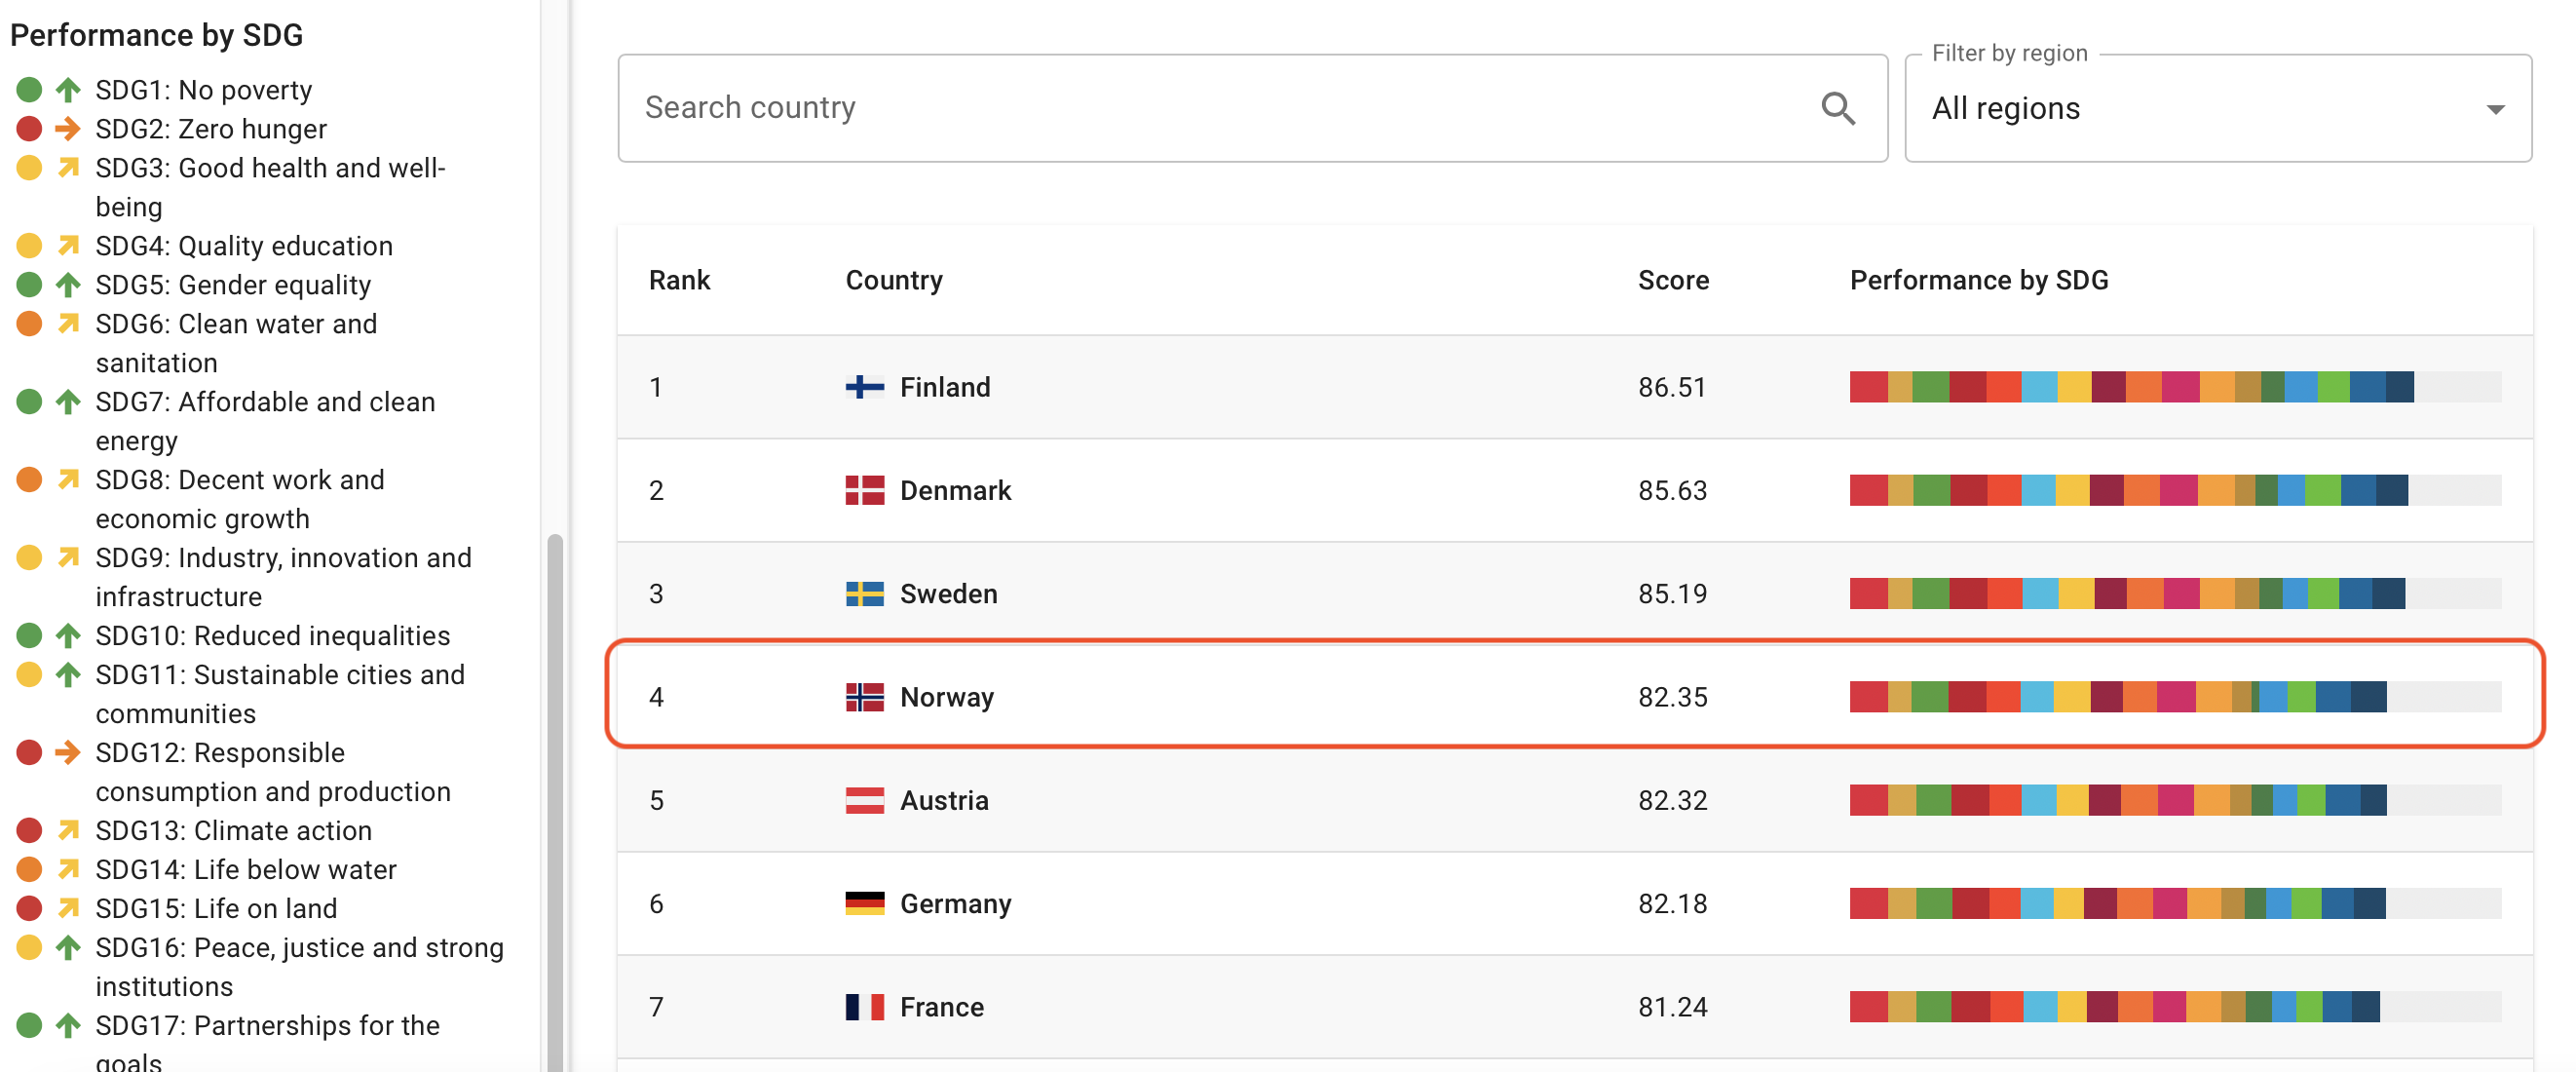
\includegraphics[scale=0.3]{figures/sdg.png}  % largura percentual
	   \caption{SDG Index Report, source: \href{https://dashboards.sdgindex.org/rankings}{SDG Index}}
	   \label{fig:sdg}
    \end{figure}

As for Alaska:

\begin{flushright}
   \textsl{''This cash has reduced income inequality in Alaska to the lowest level in America in 2016.'' \cite{huffpost}} \\
\end{flushright}

\begin{comment}
    \vspace*{1cm}
        Dayen, D., "Alaska Gives Cash To Its Citizens Every Year. The Rest Of The U.S. Could Too", \href{https://www.huffpost.com/entry/sovereign-wealth-fund-for-america-alaska-norway_n_5b83ffb7e4b0cd327dfe878e}{HuffPost}
\end{comment}

And its Gini coefficient\footnote{"The Gini coefficient measures the extent to which the distribution of income within a country deviates from a perfectly equal distribution. A coefficient of 0 expresses perfect equality where everyone has the same income, while a coefficient of 100 expresses full inequality where only one person has all the income."- Source: \href{https://ec.europa.eu/eurostat/statistics-explained/index.php?title=Glossary:Gini_coefficient}{Europa- Statistics Explained}}:

\begin{flushright}
   \textsl{''The Gini coefficient in Alaska is 0.438 — lower than the national average and fifth lowest among all 50 states.'' \cite{247}} \\

\end{flushright}

\begin{comment}
    \vspace*{1cm}
        Stebbins, S., "How Income Inequality in Alaska Compares to Other States", \href{https://247wallst.com/state/how-income-inequality-in-alaska-compares-to-other-states/}{24/7 Wall Street}
\end{comment}

However, although that's a great start, Norway and Alaska only shares the profits of mineral wealth. And, nowadays, wealth can be generated from multiple sources.\newline


    \item \textbf{The Promise of Cryptocurrency and Blockchain Technology}


Cryptocurrencies have emerged as alternative digital currencies that operate on decentralized networks. Built on blockchain technology, cryptocurrencies offer unique features that have the potential to address some of the challenges posed by traditional financial systems. These features include transparency, immutability and accessibility. By eliminating intermediaries, cryptocurrencies provide individuals with greater control over their finances and facilitate global financial inclusion \cite{twp, cwi, coint}.

As for blockchain itself:

\begin{flushright}
   \textsl{''The idea of the sharing economy has so far come from companies like Airbnb, Uber and Lyft and has been controlled by venture capital-backed private corporations. Here’s where blockchain comes in:[...] each new robot in an autonomous vehicle fleet could be fractionally owned by every member of the community in which it operates. Every time someone purchased a ride with one of the vehicles, rather than the income only going to a private company, it could be distributed to everyone in the community.'' \cite{twp}} \\

\end{flushright}

\begin{comment}
    \vspace*{1cm}
        "Here’s how blockchain can reduce inequality", \href{https://www.washingtonpost.com/news/theworldpost/wp/2018/01/29/blockchain/}{The Washington Post}
\end{comment}

This type of reaction towards income inequality can be the brake the world needs:

\begin{flushright}
   \textsl{''Instead of waiting for the inequality to happen and then addressing it via a universal basic income, we can instead pursue the idea of a universal right to intellectual and capital goods — a universal basic capital.''} \cite{twp} \\

\end{flushright}

\begin{comment}
    \vspace*{1cm}
        "Here’s how blockchain can reduce inequality", \href{https://www.washingtonpost.com/news/theworldpost/wp/2018/01/29/blockchain/}{The Washington Post}
\end{comment}

    \item \textbf{Decentralized Finance: Empowering Financial Freedom}

    Decentralized finance builds upon the foundation of cryptocurrencies and blockchain by creating a suite of financial services and applications that are accessible to anyone with an Internet connection. Through smart contracts, decentralized lending platforms and decentralized exchanges, DeFi enables individuals to borrow, lend, trade and invest without relying on traditional financial institutions. This democratizes access to financial services and empowers individuals, particularly those in underserved communities, to participate in the global economy \cite{twp, cwi, coint}.

    \item \textbf{Tackling Global Income Inequality through DeFi}

    Can decentralized finance truly address global income inequality? While it is not a \textit{panacea}\footnote{Panacea comes from the greek \textit{Panacea}, the goddess of healing, and it's used as a term to define "the universal cure".}, DeFi has the potential to make a significant impact. By providing accessible and affordable financial services, DeFi can empower individuals in low-income communities to access capital, build businesses and improve their economic prospects. Additionally, decentralized finance reduces the barriers to entry for investment and wealth accumulation, allowing individuals to participate in previously exclusive financial markets \cite{twp, cwi, coint}.

    
\end{enumerate}


\subsection{How Dharma Network works}

Dharma Network's token, DHARM, comes as a way of tackling that inequality by, in a way, giving the worker a bonus depending on the work developed. The more and the better their work is, the more they earn.\newline

Dharma Network is accessed through a decentralized application, or DApp.\newline

Dharma Network facilitates lending and borrowing activities between users. Individuals can lend their digital assets to others and earn interest on their holdings. Borrowers, on the other hand, can access these funds by collateralizing their own digital assets. This peer-to-peer lending and borrowing model eliminates the need for intermediaries such as banks \cite{dharma}.\newline

Smart contracts (see section \ref{sc}) handle the transfer of funds, collateral management and interest payments.\newline

Borrowers on Dharma Network are required to provide collateral to secure their loans. The value of the collateral should be sufficient to cover the borrowed amount. This reduces the risk for lenders, as they have collateral to claim in case of default. Collateral is stored in smart contracts and released once the borrowed amount is repaid.\newline

Dharma Network allows lenders to set their own interest rates, creating a competitive and transparent lending environment. Borrowers can choose among available loan offers based on their preferences and the interest rates offered by lenders. The interest rates are determined by market demand and supply dynamics.\newline

Dharma Network provides a governance framework that allows users to have an equal voice in the decision-making process. This means that all users, regardless of their holding size, can participate in shaping the future of the platform. Users can vote on proposals and contribute to the development and evolution of Dharma Network \cite{dharma}.\newline

The platform is designed to be user-friendly and secure, ensuring that users can confidently engage in every activity.\newline

As for the first implementation of Dharma Network, it works as a regular cryptocurrency token, being earned manually by purchasing it. However, DHARM will soon (see chapter \ref{chap:chap4}) work as a reward token, as mentioned previously.\newline

Such concepts as Smart Contracts, Blockchain, DeFi and even Dharma Network and its token, DHARM, will be detailed in the next chapter (chapter \ref{chap:sota}) of this document.

\section{Work Plan} \label{sec:plan}

The development of Dharma Network follows a comprehensive work plan. The backend services are primarily built using Elixir, a robust and scalable programming language and the Phoenix framework. Additionally, Python is utilized for various integrations and data processing tasks. Leveraging the Algorand blockchain, Dharma Network ensures a secure and decentralized environment for users.

\section{Document Structure} \label{sec:struct}

The presented document is split into 6 chapters, with an additional appendix at the end:

\begin{itemize}
    \item Chapter 1- includes the objectives of the work, its context and used methodology;
	\item Chapter 2- describes the state of the art, the tools used, important concepts and related work;
	\item Chapter 3- contains a detailed description of the developed work and analysis of the requirements, such as the study objects;
	\item  Chapter 4- includes the developed work for Dharma Network, as well as other relevant information;
	\item Chapter 5- contains the analysis of the results, such as a comparison between the initial sprint planning and the execution of such sprints;
	\item Chapter 6- includes a summary of the work, a critical commentary and a discussion of future work that could be an improvement to the existing platform.
\end{itemize}


\subsection{Work Considerations}

Some considerations to have about the work are:

\begin{itemize} 

	\item The main work focus is the backend of Dharma Network;
	\item Methodology \textbf{Scrum}\footnote{\href{https://www.atlassian.com/agile/scrum}{Scrum} is an agile project management methodology that helps teams structure and manage their work} will be used for project planning;
	\item The chosen working repository is GitHub, where the project's version control will also be done;
	\item This document is organised and described in the document structure;
	\item The organisation dossier will be on chapter \ref{sprint} and Appendix of this document.
\end{itemize}